    \hypertarget{construction-de-liste-par-compruxe9hension}{%
\section{Construction de liste par
compréhension}\label{construction-de-liste-par-compruxe9hension}}

    \hypertarget{ruxe9vision---niveau-basique}{%
\subsection{Révision - niveau
basique}\label{ruxe9vision---niveau-basique}}

    Ce mécanisme très pratique permet de construire simplement une liste à
partir d'une autre (ou de \textbf{tout autre type itérable} en réalité,
mais nous y viendrons).

Pour l'introduire en deux mots, disons que la compréhension de liste est
à l'instruction \texttt{for} ce que l'expression conditionnelle est à
l'instruction \texttt{if}, c'est-à-dire qu'il s'agit d'une
\textbf{expression à part entière}.

    \hypertarget{cas-le-plus-simple}{%
\subsubsection{Cas le plus simple}\label{cas-le-plus-simple}}

    Voyons tout de suite un exemple~:

    \begin{Verbatim}[commandchars=\\\{\}]
{\color{incolor}In [{\color{incolor}1}]:} \PY{n}{depart} \PY{o}{=} \PY{p}{(}\PY{o}{\PYZhy{}}\PY{l+m+mi}{5}\PY{p}{,} \PY{o}{\PYZhy{}}\PY{l+m+mi}{3}\PY{p}{,} \PY{l+m+mi}{0}\PY{p}{,} \PY{l+m+mi}{3}\PY{p}{,} \PY{l+m+mi}{5}\PY{p}{,} \PY{l+m+mi}{10}\PY{p}{)}
        \PY{n}{arrivee} \PY{o}{=} \PY{p}{[}\PY{n}{x}\PY{o}{*}\PY{o}{*}\PY{l+m+mi}{2} \PY{k}{for} \PY{n}{x} \PY{o+ow}{in} \PY{n}{depart}\PY{p}{]}
        \PY{n}{arrivee}
\end{Verbatim}


\begin{Verbatim}[commandchars=\\\{\}]
{\color{outcolor}Out[{\color{outcolor}1}]:} [25, 9, 0, 9, 25, 100]
\end{Verbatim}
            
    Le résultat de cette expression est donc une liste, dont les éléments
sont les résultats de l'expression \texttt{x**2} pour \texttt{x} prenant
toutes les valeurs de \texttt{depart}.

    \textbf{Remarque}~: si on prend un point de vue un peu plus
mathématique, ceci revient donc à appliquer une certaine fonction (ici
\(x \rightarrow x^2\)) à une collection de valeurs, et à retourner la
liste des résultats. Dans les langages fonctionnels, cette opération est
connue sous le nom de \texttt{map}, comme on l'a vu dans la séquence
précédente.

    \hypertarget{digression}{%
\subparagraph{Digression}\label{digression}}

    \begin{Verbatim}[commandchars=\\\{\}]
{\color{incolor}In [{\color{incolor}2}]:} \PY{c+c1}{\PYZsh{} profitons de cette occasion pour voir }
        \PY{c+c1}{\PYZsh{} comment tracer une courbe avec matplotlib}
        \PY{o}{\PYZpc{}}\PY{k}{matplotlib} inline
        \PY{k+kn}{import} \PY{n+nn}{matplotlib}\PY{n+nn}{.}\PY{n+nn}{pyplot} \PY{k}{as} \PY{n+nn}{plt}
        \PY{n}{plt}\PY{o}{.}\PY{n}{ion}\PY{p}{(}\PY{p}{)}
\end{Verbatim}


    \begin{Verbatim}[commandchars=\\\{\}]
{\color{incolor}In [{\color{incolor}3}]:} \PY{c+c1}{\PYZsh{} si on met le départ et l\PYZsq{}arrivée }
        \PY{c+c1}{\PYZsh{} en abscisse et en ordonnée, on trace}
        \PY{c+c1}{\PYZsh{} une version tronquée de la courbe de f: x \PYZhy{}\PYZgt{} x**2}
        \PY{n}{plt}\PY{o}{.}\PY{n}{plot}\PY{p}{(}\PY{n}{depart}\PY{p}{,} \PY{n}{arrivee}\PY{p}{)}\PY{p}{;}
\end{Verbatim}


    \begin{center}
 	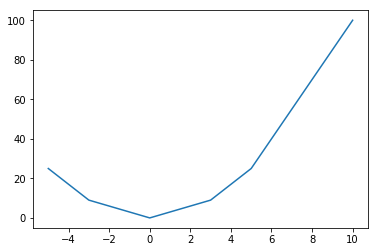
\includegraphics{medias/output_11_0.png}  
    \end{center}
    { \hspace*{\fill} \\}
 
    \hypertarget{restriction-uxe0-certains-uxe9luxe9ments}{%
\subsubsection{Restriction à certains
éléments}\label{restriction-uxe0-certains-uxe9luxe9ments}}

    Il est possible également de ne prendre en compte que certains des
éléments de la liste de départ, comme ceci~:

    \begin{Verbatim}[commandchars=\\\{\}]
{\color{incolor}In [{\color{incolor}4}]:} \PY{p}{[}\PY{n}{x}\PY{o}{*}\PY{o}{*}\PY{l+m+mi}{2} \PY{k}{for} \PY{n}{x} \PY{o+ow}{in} \PY{n}{depart} \PY{k}{if} \PY{n}{x}\PY{o}{\PYZpc{}}\PY{k}{2} == 0]
\end{Verbatim}


\begin{Verbatim}[commandchars=\\\{\}]
{\color{outcolor}Out[{\color{outcolor}4}]:} [0, 100]
\end{Verbatim}
            
    qui cette fois ne contient que les carrés des éléments pairs de
\texttt{depart}.\\

    \textbf{Remarque}~: pour prolonger la remarque précédente, cette
opération s'appelle fréquemment \texttt{filter} dans les langages de
programmation.

    \hypertarget{autres-types}{%
\subsubsection{Autres types}\label{autres-types}}

    On peut fabriquer une compréhension à partir de tout objet itérable, pas
forcément une liste, mais le résultat est toujours une liste, comme on
le voit sur ces quelques exemples~:

    \begin{Verbatim}[commandchars=\\\{\}]
{\color{incolor}In [{\color{incolor}5}]:} \PY{p}{[}\PY{n+nb}{ord}\PY{p}{(}\PY{n}{x}\PY{p}{)} \PY{k}{for} \PY{n}{x} \PY{o+ow}{in} \PY{l+s+s1}{\PYZsq{}}\PY{l+s+s1}{abc}\PY{l+s+s1}{\PYZsq{}}\PY{p}{]}
\end{Verbatim}


\begin{Verbatim}[commandchars=\\\{\}]
{\color{outcolor}Out[{\color{outcolor}5}]:} [97, 98, 99]
\end{Verbatim}
            
    \begin{Verbatim}[commandchars=\\\{\}]
{\color{incolor}In [{\color{incolor}6}]:} \PY{p}{[}\PY{n+nb}{chr}\PY{p}{(}\PY{n}{x}\PY{p}{)} \PY{k}{for} \PY{n}{x} \PY{o+ow}{in} \PY{p}{(}\PY{l+m+mi}{97}\PY{p}{,} \PY{l+m+mi}{98}\PY{p}{,} \PY{l+m+mi}{99}\PY{p}{)}\PY{p}{]}
\end{Verbatim}


\begin{Verbatim}[commandchars=\\\{\}]
{\color{outcolor}Out[{\color{outcolor}6}]:} ['a', 'b', 'c']
\end{Verbatim}
            
    \hypertarget{autres-types-2}{%
\subsubsection{Autres types (2)}\label{autres-types-2}}

    On peut également construire par compréhension des dictionnaires et des
ensembles~:

    \begin{Verbatim}[commandchars=\\\{\}]
{\color{incolor}In [{\color{incolor}7}]:} \PY{n}{d} \PY{o}{=} \PY{p}{\PYZob{}}\PY{n}{x}\PY{p}{:} \PY{n+nb}{ord}\PY{p}{(}\PY{n}{x}\PY{p}{)} \PY{k}{for} \PY{n}{x} \PY{o+ow}{in} \PY{l+s+s1}{\PYZsq{}}\PY{l+s+s1}{abc}\PY{l+s+s1}{\PYZsq{}}\PY{p}{\PYZcb{}}
        \PY{n}{d}
\end{Verbatim}


\begin{Verbatim}[commandchars=\\\{\}]
{\color{outcolor}Out[{\color{outcolor}7}]:} \{'a': 97, 'b': 98, 'c': 99\}
\end{Verbatim}
            
    \begin{Verbatim}[commandchars=\\\{\}]
{\color{incolor}In [{\color{incolor}8}]:} \PY{n}{e} \PY{o}{=} \PY{p}{\PYZob{}}\PY{n}{x}\PY{o}{*}\PY{o}{*}\PY{l+m+mi}{2} \PY{k}{for} \PY{n}{x} \PY{o+ow}{in} \PY{p}{(}\PY{l+m+mi}{97}\PY{p}{,} \PY{l+m+mi}{98}\PY{p}{,} \PY{l+m+mi}{99}\PY{p}{)} \PY{k}{if} \PY{n}{x} \PY{o}{\PYZpc{}}\PY{k}{2} == 0\PYZcb{}
        \PY{n}{e}
\end{Verbatim}


\begin{Verbatim}[commandchars=\\\{\}]
{\color{outcolor}Out[{\color{outcolor}8}]:} \{9604\}
\end{Verbatim}
            
    \hypertarget{pour-en-savoir-plus}{%
\subsubsection{Pour en savoir plus}\label{pour-en-savoir-plus}}

    Voyez
\href{https://docs.python.org/3/tutorial/datastructures.html\#list-comprehensions}{la
section sur les compréhensions de liste} dans la documentation python.